% Created 2022-11-16 mer 14:30
% Intended LaTeX compiler: pdflatex
\documentclass[presentation]{beamer}
\usepackage[utf8]{inputenc}
\usepackage[T1]{fontenc}
\usepackage{graphicx}
\usepackage{longtable}
\usepackage{wrapfig}
\usepackage{rotating}
\usepackage[normalem]{ulem}
\usepackage{amsmath}
\usepackage{amssymb}
\usepackage{capt-of}
\usepackage{hyperref}
\usepackage{minted}
\usepackage[, french]{babel}
\usepackage{svg}
\logo{
\includegraphics[width=.1\textwidth]{../../by-sa.png}}
\usetheme{metropolis}
\usecolortheme{}
\usefonttheme{}
\useinnertheme{}
\useoutertheme{}
\author{Guy Bégin}
\date{\today}
\title{Circuits logiques combinatoires et séquentiels}

\hypersetup{
 pdfauthor={Guy Bégin},
 pdftitle={Circuits logiques combinatoires et séquentiels},
 pdfkeywords={},
 pdfsubject={},
 pdfcreator={Emacs 28.1 (Org mode 9.5.4)}, 
 pdflang={French}}
\begin{document}

\maketitle

\section{Systèmes de numération}
\label{sec:org40742a2}


\begin{frame}[label={sec:org84e2220}]{Objectifs}
\begin{itemize}
\item Comprendre le fonctionnement du système de numération binaire
\item Pouvoir effectuer des conversions entre nombres en représentation
binaire, octale, hexadécimale
\item Comprendre le rôle des compléments, et la représentation de nombres signés
\item Comprendre la notation fractionnaire
\item Se familiariser avec quelques codes courants
\item Pouvoir effectuer des opérations arithmétiques sur des nombres binaires
\end{itemize}
\end{frame}

\begin{frame}[label={sec:org097f489}]{Systèmes numériques}
\begin{itemize}
\item Les systèmes numériques sont omniprésents dans notre monde technologique.

\item La grande force des systèmes numériques est leur capacité à représenter l'information sous toutes ses formes et à permettre la manipulation de cette information.

\item Tout ensemble dont les éléments peuvent être dénombrés, comme un alphabet ou un ensemble fini de couleurs, se prête naturellement à une représentation numérique.

\item Mais il est également possible de représenter des informations qui correspondent à des informations provenant d'ensembles continus, comme par exemple des informations sonores, en procédant à une numérisation par échantillonnage et codage.
\end{itemize}
\end{frame}

\begin{frame}[label={sec:orgf58a2b9}]{Systèmes numériques \ldots{} 2}
\begin{itemize}
\item Une bonne façon de se familiariser avec la représentation numérique de l'information est d'étudier le système de numération binaire.

\item Dans un chapitre suivant, nous étudierons les principes fondamentaux de la logique binaire.

\item C'est sur ces deux bases que nous pourrons établir notre exploration des circuits logiques.
\end{itemize}
\end{frame}

\begin{frame}[label={sec:org9c73ec7}]{Nombres binaires}
\begin{itemize}
\item Les nombres binaires sont essentiellement construits de la même façon que les nombres décimaux avec lesquels nous sommes plus familiers.

\item La différence fondamentale tient au fait qu'il n'est possible d'utiliser que deux symboles (chiffres), 0 et 1, plutôt que les dix chiffres de 0 à 9.

\item Les chiffres sont nommés bits (contraction de \alert{b} inary dig \alert{it}).
\end{itemize}
\end{frame}

\begin{frame}[label={sec:org341a92e}]{Nombres binaires \ldots{} 2}
\begin{itemize}
\item Par exemple, le nombre décimal que nous écrivons \(2843\) correspond à \(2 \times 1000 + 8 \times 100 + 4 \times 10 + 3 \times 1\).

\item Il s'agit d'un système positionnel, dans lequel la valeur attribuée à un chiffre est définie par sa position et par la valeur de la \alert{base} du système de numération.

\item Ainsi, pour ce nombre décimal, la base vaut 10 et on a \(2 \times 10^3 + 8 \times 10^2 + 4 \times 10^1 + 3 \times 10^0\).
\end{itemize}
\end{frame}

\begin{frame}[label={sec:org8e454ca}]{Nombres binaires \ldots{} 3}
\begin{itemize}
\item La position la plus à gauche est celle dont la valeur est la plus grande.

\item C'est le \alert{chiffre le plus significatif}; la position de droite correspond au \alert{chiffre le moins significatif}.

\item On peut imaginer une virgule après le chiffre le moins significatif, pour délimiter la partie entière du nombre.

\item D'autres chiffres, placés à droite de cette virgule correspondraient à la partie fractionnaire.  On y reviendra.
\end{itemize}
\end{frame}

\begin{frame}[label={sec:org36f7f94}]{Nombres binaires \ldots{} 4}
\begin{itemize}
\item Les mêmes règles positionnelles permettent d'attribuer une valeur à un nombre binaire, en tenant compte du fait que la base vaut cette fois-ci 2.

\item Par exemple, la valeur attribuée au nombre binaire \(10101\) est

$$ 1 \times 2^4 + 0 \times 2^3 + 1 \times 2^2 + 0 \times 2^1 + 1 \times 2^0 = 16+4+1= 21 $$
\end{itemize}

comme on peut voir dans le tableau \ref{tab:orgdd880d8}.
\end{frame}

\begin{frame}[label={sec:org089edbb}]{Nombres binaires \ldots{} 5}
\begin{table}[htbp]
\caption{\label{tab:orgdd880d8}Valeur binaire du nombre \(10101\)}
\centering
\begin{tabular}{lrrrrr}
Position & 4 & 3 & 2 & 1 & 0\\
\hline
Valeur & \(2^4\) & \(2^3\) & \(2^2\) & \(2^1\) & \(2^0\)\\
Valeur déc. & 16 & 8 & 4 & 2 & 1\\
Bit & 1 & 0 & 1 & 0 & 1\\
\end{tabular}
\end{table}

\begin{itemize}
\item Nous avons ici le \alert{bit le plus significatif} à gauche et le \alert{bit le moins significatif} à droite.

\item Chaque chiffre vaut 2 fois plus que le chiffre immédiatement placé à sa droite.
\end{itemize}
\end{frame}

\begin{frame}[label={sec:orgcd5028c}]{Conversion binaire <-> décimal}
\begin{itemize}
\item Convertir un nombre entier binaire en nombre décimal se fait naturellement, en s'appuyant sur les valeurs associées à la notation positionnelle.

\item La conversion en sens inverse, de décimal à binaire, est un peu moins évidente.
\end{itemize}
\end{frame}

\begin{frame}[label={sec:orge3f9f8b}]{Conversion binaire <-> décimal \ldots{} 2}
\begin{itemize}
\item La méthode consiste à faire une division entière du nombre (et des quotients successifs) par 2 et à noter les restes obtenus.

\item Le premier reste correspond au bit le moins significatif, et le dernier au bit le plus significatif.
\end{itemize}
\end{frame}

\begin{frame}[label={sec:org0ee896a}]{Conversion binaire <-> décimal \ldots{} 3}
\begin{itemize}
\item Par exemple, les opération pour convertir 37 en binaire sont résumées dans le tableau \ref{tab:org7d453e6}.
\end{itemize}

\begin{table}[htbp]
\caption{\label{tab:org7d453e6}Étapes de conversion de 37 en binaire}
\centering
\begin{tabular}{lrrl}
 & Quotient entier & Reste & Coefficient\\
\hline
37/2 & 18 & 1 & \(a_0 = 1\)\\
18/2 & 9 & 0 & \(a_1 = 0\)\\
9/2 & 4 & 1 & \(a_2 = 1\)\\
4/2 & 2 & 0 & \(a_3 = 0\)\\
2/2 & 1 & 0 & \(a_4 = 0\)\\
1/2 & 0 & 1 & \(a_5 = 1\)\\
\end{tabular}
\end{table}

On obtient ainsi 100101.
\end{frame}

\begin{frame}[label={sec:orgf14f2f6}]{Notation}
\begin{itemize}
\item Puisque les notations de nombres binaires, octaux, hexadécimaux ou décimaux font appel à des chiffres qui sont tous tirés du même ensemble, il y a un risque d’ambiguïté si on ne connaît pas la base utilisée.

\item Par exemple 11 peut soit s'interpréter comme onze (si on suppose la base dix) ou comme trois (si on suppose la base deux).

\item À moins que le contexte ne soit absolument clair, il vaut mieux être explicite pour éviter de telles ambiguïtés.
\end{itemize}
\end{frame}

\begin{frame}[label={sec:org91925cc}]{Notation \ldots{} 2}
\begin{itemize}
\item C'est pourquoi on dénote souvent explicitement la base, comme par exemple, (11)2 pour le nombre trois en binaire qui pourra être distingué de (11)10, le nombre onze en décimal.
\end{itemize}
\end{frame}

\begin{frame}[label={sec:org937e747}]{Représentations compactes de nombres binaires}
\begin{itemize}
\item En comparant un nombre décimal et sa représentation binaire, comme par exemple ici 37 et 100101, on voit bien que la représentation binaire est nettement plus encombrante

\item On utilise souvent des notations plus compactes mais qui conservent un lien direct avec la représentation binaire: la représentation \alert{octale} et la représentation \alert{hexadécimale}.
\end{itemize}
\end{frame}

\begin{frame}[label={sec:org14ff5b2}]{Représentation octale}
\begin{columns}
\begin{column}{0.48\columnwidth}
\begin{block}{Notation octale}
\begin{itemize}
\item La représentation octale correspond à utiliser la base 8, avec les chiffres \(0, 1, \ldots, 7\)

\item On voit la correspondance entre les nombres en binaire et les chiffres de la représentation octale dans le tableau \ref{tab:org224cab8}.
\end{itemize}
\end{block}
\end{column}

\begin{column}{0.48\columnwidth}
\begin{block}{}
\begin{table}[htbp]
\caption{\label{tab:org224cab8}Représentation octale}
\centering
\begin{tabular}{rr}
Binaire & Octal\\
\hline
000 & 0\\
001 & 1\\
010 & 2\\
011 & 3\\
100 & 4\\
101 & 5\\
110 & 6\\
111 & 7\\
\end{tabular}
\end{table}
\end{block}
\end{column}
\end{columns}
\end{frame}

\begin{frame}[label={sec:orge620a0f}]{Représentation octale \ldots{} 2}
\begin{itemize}
\item Pour convertir un nombre binaire en nombre octal, il suffit de regrouper les bits par groupes de trois bits, en partant de la droite (bit le moins significatif), et de remplacer chaque groupe par le chiffre en base 8 correspondant.

\item Par exemple pour (1010011110001)2, on aura le découpage du tableau \ref{tab:org211dc88}.
\end{itemize}

\begin{table}[htbp]
\caption{\label{tab:org211dc88}Regroupement pour conversion en octal}
\centering
\begin{tabular}{lrrrrr}
 &  &  &  &  & \\
\hline
Binaire & 1 & 010 & 011 & 110 & 001\\
Octal & 1 & 2 & 3 & 6 & 1\\
\end{tabular}
\end{table}

\begin{itemize}
\item On obtient le nombre octal (12361)8.
\end{itemize}
\end{frame}

\begin{frame}[label={sec:org71fc0ec}]{Représentation hexadécimale}
\begin{itemize}
\item La représentation hexadécimale correspond à utiliser la base 16, avec les chiffres \(0, 1, \ldots, 9\), auxquels on ajoute les lettres A, B, C, D, E et F pour représenter les valeurs de dix à quinze respectivement.

\item Pour simplifier, dans le contexte, on appellera ici ces cinq lettres des \emph{chiffres} de la notation hexadécimale.

\item On voit la correspondance entre les nombres en binaire et les chiffres de la représentation hexadécimale dans le tableau \ref{tab:orgfadd90d}.
\end{itemize}
\end{frame}


\begin{frame}[label={sec:org08960a1}]{Représentation hexadécimale \ldots{} 2}
\begin{columns}
\begin{column}{0.48\columnwidth}
\begin{block}{}
\begin{table}[htbp]
\caption{\label{tab:orgfadd90d}Représentation hexadécimale}
\centering
\begin{tabular}{rr}
Binaire & Hexadécimal\\
\hline
0000 & 0\\
0001 & 1\\
0010 & 2\\
0011 & 3\\
0100 & 4\\
0101 & 5\\
0110 & 6\\
0111 & 7\\
\end{tabular}
\end{table}
\end{block}
\end{column}

\begin{column}{0.48\columnwidth}
\begin{block}{}
\begin{center}
\begin{tabular}{rl}
Binaire & Hexadécimal\\
\hline
1000 & 8\\
1001 & 9\\
1010 & A\\
1011 & B\\
1100 & C\\
1101 & D\\
1110 & E\\
1111 & F\\
\end{tabular}
\end{center}
\end{block}
\end{column}
\end{columns}
\end{frame}

\begin{frame}[label={sec:org666ae3f}]{Représentation hexadécimale \ldots{} 3}
\begin{itemize}
\item Pour convertir un nombre binaire en nombre hexadécimal, il suffit de regrouper les bits par groupes de quatre bits, en partant de la droite (bit le moins significatif), et de remplacer chaque groupe par le chiffre en base 16 correspondant

\item Par exemple pour (1010011110001)2, on aura le découpage du tableau \ref{tab:org5ce7a0f}.
\end{itemize}

\begin{table}[htbp]
\caption{\label{tab:org5ce7a0f}Regroupement pour conversion en hexadécimal}
\centering
\begin{tabular}{lrrrr}
 &  &  &  & \\
\hline
Binaire & 1 & 0100 & 1111 & 0001\\
Hexa & 1 & 4 & F & 1\\
\end{tabular}
\end{table}

\begin{itemize}
\item On obtient le nombre hexadécimal (14F1)16.
\end{itemize}
\end{frame}

\begin{frame}[label={sec:orgcd1d46e}]{Conversion en sens inverse}
\begin{itemize}
\item La conversion de octal (respectivement, hexadécimal) à binaire se fait simplement en remplaçant chaque chiffre octal (resp., hexadécimal) par le groupe de trois (resp., quatre) bits correspondant, en partant du moins significatif.
\end{itemize}
\end{frame}

\begin{frame}[label={sec:org5007741}]{Nombres binaires fractionnaires}
\begin{itemize}
\item Il est aussi possible de représenter des nombres fractionnaires en base deux.

\item En gardant à l'esprit que la position d'un bit détermine sa valeur, il suffit d'étendre le principe déjà établi aux bits qui seront placés après la virgule qui sépare la partie entière de la partie fractionnaire.

\item Les indices des positions à droite de la virgule seront négatifs.

\item Le tableau \ref{tab:orgb5909a7} donne par exemple le détail de l'évaluation de la valeur du nombre fractionnaire (101,11)2.

\item On obtient comme valeur \(1 \times 4 + 0 \times 2 + 1 \times 1 + 1 \times 1/2 + 1 \times 1/4 = 5,75\).
\end{itemize}
\end{frame}

\begin{frame}[label={sec:org199441b}]{Nombres binaires fractionnaires \ldots{} 2}
\begin{table}[htbp]
\caption{\label{tab:orgb5909a7}Évaluation de la valeur du nombre fractionnaire (101,11)2}
\centering
\begin{tabular}{lrrrrr}
Position & 2 & 1 & 0 & -1 & -2\\
\hline
Valeur & \(2^2\) & \(2^1\) & \(2^0\) & \(2^{-1}\) & \(2^{-2}\)\\
Valeur déc. & 4 & 2 & 1 & 1/2 & 1/4\\
Bit & 1 & 0 & 1 & 1 & 1\\
\end{tabular}
\end{table}
\end{frame}

\begin{frame}[label={sec:org89e4352}]{Opérations arithmétiques binaires}
\begin{itemize}
\item Il est possible de transposer les opérations arithmétiques habituelles pour effectuer différentes opération arithmétiques: addition, soustraction, multiplication, division, avec des nombres binaires.

\item Nous verrrons plus loin comment ces opérations s'exécutent lorsque nous aurons établi les formes d'encodages binaires qui seront utilisés pour les nombres, notamment la représentation des nombres signés.
\end{itemize}
\end{frame}

\begin{frame}[label={sec:org51d265c}]{Multiplication par deux}
\begin{itemize}
\item Pour multiplier un nombre binaire non signé par deux, il suffit de décaler tous ses bits d'une position vers la gauche.

\item Si le nombre est entier, on devra insérer un zéro à la position zéro.

\item Si le nombre est fractionnaire, le bit le plus significatif de la partie fractionnaire se retrouvera à la position zéro.

$$ (10011)2 \times 2 = (100110)2 $$

$$ (100,11)2 \times 2 = (1001,1)2 $$
\end{itemize}
\end{frame}

\begin{frame}[label={sec:org7e7af90}]{Division par deux: fractionnaire}
\begin{itemize}
\item Pour diviser un nombre binaire par deux, il suffit de décaler tous ses bits d'une position vers la droite.

\item Une division fractionnaire produira possiblement un nombre fractionnaire, comme dans l'exemple suivant.
\end{itemize}


$$ (10011)2 \div 2 = (1001,1)2 $$
\end{frame}

\begin{frame}[label={sec:orgf3676f8}]{Division par deux: entière}
\begin{itemize}
\item Pour une division entière (sans fraction), on éliminera le bit qui aurait été placé après la virgule.

$$ (10011)2 \div 2 = (1001)2 $$

\item Il est évident de généraliser ces opérations pour les multiplications ou divisions par des puissances de 2: par 4, 8, 16, etc.
\end{itemize}
\end{frame}


\begin{frame}[label={sec:orgaae5dea}]{Compléments de nombres}
\begin{itemize}
\item Les compléments de nombres jouent un rôle dans la simplification de certaines opérations mathématiques et logiques.

\item Dans un système de numération de base \(b\), on considère deux types de compléments: le complément à \(b\) et le complément à \(b-1\).

\item Pour la base dix, nous aurons donc le complément à dix et le complément à neuf.

\item Pour les nombres binaires (base 2), on aura le complément à deux et le complément à un.

\item Pour évaluer les compléments d'un nombre, on doit tenir compte du nombre de chiffres que comporte ce nombre.
\end{itemize}
\end{frame}

\begin{frame}[label={sec:org70fda31}]{Complément à neuf}
\begin{itemize}
\item Soit un nombre entier \(N\) en base \(b\) constitué de \(n\) chiffres.

\item Le complément à \(b-1\) de \(N\) est \((b^n-1)-N\).

\item Par exemple, en base \(b=10\), le complément à neuf pour le nombre décimal \(N = 4576\) formé de \(n=4\) chiffres sera \((b^n-1)-N = (10^4 -1) - 4576 = 5424\).
\end{itemize}
\end{frame}

\begin{frame}[label={sec:org67be6ee}]{Complément à un}
\begin{itemize}
\item En base \(b=2\), le complément à un pour le nombre binaire \(N = (10011)2 = (19)10\) formé de \(n=5\) bits sera \((b^n-1)-N = (2^5 -1) - 19 = 12\) ce qui donne en binaire: \((12)10 = (1100)2\).

\item On peut vérifier qu'il est très facile, en binaire, de déterminer le complément à un, sans effectuer de calculs, en inversant simplement chacun des bits de la représentation binaire du nombre à complémenter.

\item Ainsi, avec notre exemple, on trouve pour  $$ 10011 $$ le complément $$ 01100 $$

\item Remarquons ici un zéro non significatif comme premier bit à gauche.
\end{itemize}
\end{frame}

\begin{frame}[label={sec:org28fdcfe}]{Complément à dix}
\begin{itemize}
\item Le complément à \(b\) de l'entier \(N\) s'évalue comme \((b^n)-N\).

\item Cela correspond à ajouter 1 au complément à \(b-1\).

\item Ainsi pour notre exemple précédent en base \(b=10\), le complément à dix pour le nombre décimal \(N = 4576\) formé de \(n=4\) chiffres sera \((b^n)-N = (10^4) - 4576 = 5425\).
\end{itemize}
\end{frame}

\begin{frame}[label={sec:org58fd942}]{Complément à deux}
\begin{itemize}
\item Pour notre autre exemple, en base \(b=2\), le complément à deux pour le nombre binaire \(N = (10011)2 = (19)10\) formé de \(n=5\) bits sera \((b^n)-N = (2^5) - 19 = 13\) ce qui donne en binaire: \((13)10 = (1101)2\).
\end{itemize}
\end{frame}

\begin{frame}[label={sec:orgb8afa2a}]{Complément à deux \ldots{} 2}
\begin{itemize}
\item L'évaluation directe à la main, sans calculs, du complément à deux est également possible en suivant la démarche suivante:
\begin{enumerate}
\item On parcourt le nombre binaire initial à partir (à droite) du bit le moins significatif, et on retranscrit les bits rencontrés jusqu'à atteindre un premier bit 1, que l'on retranscrit également.
\item On continue la retranscription vers la gauche, en inversant cette fois les bits subséquents.
\end{enumerate}
\end{itemize}
\end{frame}

\begin{frame}[label={sec:orgc67cd51}]{Complément à deux \ldots{} 3}
\begin{itemize}
\item Par exemple, pour (10110)2, on aura la démarche détaillée dans le tableau \ref{tab:orge014b7c}.

\item Les étapes sont numérotées selon la position considérée, à partir de la droite.
\end{itemize}

\begin{table}[htbp]
\caption{\label{tab:orge014b7c}Étapes pour complément à deux}
\centering
\begin{tabular}{lrrrrrl}
Nombre & 1 & 0 & 1 & 1 & 0 & \\
\hline
Étape 0 &  &  &  &  & 0 & Retranscrit\\
Étape 1 &  &  &  & 1 & 0 & Retranscrit\\
Étape 2 &  &  & 0 & 1 & 0 & Inversé\\
Étape 3 &  & 1 & 0 & 1 & 0 & Inversé\\
Étape 4 & 0 & 1 & 0 & 1 & 0 & Inversé\\
\end{tabular}
\end{table}
\end{frame}

\begin{frame}[label={sec:org97877de}]{Complément à deux \ldots{} 4}
\begin{itemize}
\item Pour une évaluation par un circuit, on commencera par déterminer le complément à un par inversion et on lui additionnera 1 pour obtenir le complément à deux.
\end{itemize}
\end{frame}

\begin{frame}[label={sec:orgb75e1a6}]{Nombres signés et codage}
\begin{itemize}
\item Représenter de nombres \(\geq 0\) en binaire est donc relativement naturel.

\item Dans l'optique où on voudra stocker ces nombres dans une mémoire binaire numérique, il n'y a qu'à prévoir une taille suffisante (en nombre de bits) pour pouvoir accommoder des nombres assez grands pour l'application considérée.

\item Avec \(n\) bits, il est possible de représenter des entiers de 0 à \(2^n-1\) avec cette représentation «naturelle».
\end{itemize}
\end{frame}

\begin{frame}[label={sec:org662cfac}]{Nombres signés et codage \ldots{} 2}
\begin{itemize}
\item Mais on peut se demander comment représenter des nombres négatifs, c'est-à-dire \(< 0\).

\item Une première observation est le fait que si on considère des nombres positif \alert{et} négatifs, on double en quelque sorte la quantité de valeurs à représenter.
\end{itemize}
\end{frame}

\begin{frame}[label={sec:orgd261cf0}]{Nombres signés et codage \ldots{} 3}
\begin{itemize}
\item Par exemple, il y a 21 nombres à représenter si on veut pouvoir utiliser les valeurs comprises entre \(-10\) et \(+10\), comme on peut le voir dans le tableau \ref{tab:org03c9165}.
\end{itemize}

\begin{table}[htbp]
\caption{\label{tab:org03c9165}Nombre de valeurs à représenter entre \(-10\) et \(+10\)}
\centering
\begin{tabular}{lr}
Gamme & n. de valeurs\\
\hline
de -10 à -1 & 10\\
0 & 1\\
de 1 à 10 & 10\\
\hline
Total & 21\\
\end{tabular}
\end{table}

\begin{itemize}
\item Nous devons donc nous assurer d'avoir autant de combinaisons de bits qu'il sera nécessaire.
\end{itemize}
\end{frame}

\begin{frame}[label={sec:orga77e9d5}]{Nombres signés et codage \ldots{} 4}
\begin{itemize}
\item La deuxième observation est qu'il faudra un moyen de distinguer les nombres positifs des nombres négatifs.

\item Si on veut que cette distinction puisse se faire non seulement sur papier, mais surtout lorsque les nombres seront stockés et manipulés dans un système électronique, il faut définir un format binaire «tout compris» qui permette de le faire.
\end{itemize}
\end{frame}

\begin{frame}[label={sec:org83fa764}]{Nombres signés et codage \ldots{} 5}
\begin{itemize}
\item Nous devons donc établir un \alert{code}, c'est-à-dire, une \alert{convention} qui permettra de donner un sens à un groupe de bits.

\item Le choix de la convention devrait être guidé par les usages qui seront ultimement faits des nombres qui seront représentés.

\item En fait, lorsque nous avons convenu (implicitement) de représenter des nombres entiers en utilisant directement la conversion en base 2 des nombres décimaux, nous avons établi un code de représentation, qui, bien que naturel, n'en est pas moins une convention.
\end{itemize}
\end{frame}

\begin{frame}[label={sec:orgc1131e3}]{Nombres signés et codage \ldots{} 6}
\begin{itemize}
\item Ici, nous devrons formuler plus explicitement la convention qui sera utilisée pour représenter les entier signés.

\item Une convention de représentation peut être établie totalement arbitrairement, mais elle sera sans doute plus utile si elle peut contribuer à faciliter des opérations courantes réalisées avec les éléments à représenter.

\item Puisqu'il est question ici de nombre entiers signés, l'opération à considérer en priorité est l'addition.
\end{itemize}
\end{frame}

\begin{frame}[label={sec:org7eaf0b6}]{Nombres signés et convention}
\begin{itemize}
\item On devrait aussi considérer les trois points suivants dans notre choix de convention pour attribuer des codes binaires aux valeurs.

\item Pour illustrer notre réflexion, nous allons considérer des nombre pouvant être représentés par des codes binaires de quatre bits, ce qui permet en théorie de représenter un total de 16 valeurs.

\begin{enumerate}
\item Puisqu'il faudra partager notre ensemble de codes binaires en deux, il serait logique de placer la représentation pour zéro au centre de ce découpage.

\item Les codes binaires utilisés pour un nombre et pour son inverse additif devraient être disposés symétriquement autour du code utilisé pour représenter le zéro. Il est naturel de représenter la valeur zéro avec le code 0000.

\item L'ordre des codes devrait correspondre à l'ordre des nombres.
\end{enumerate}
\end{itemize}
\end{frame}

\begin{frame}[label={sec:org7427079}]{Nombres signés et convention \ldots{} 2}
\begin{itemize}
\item On sait bien comment ordonner les nombres entiers, en passant des nombres négatifs aux nombres positifs.

\item Quel ordre serait approprié pour les représentations (codes binaires)?  L'ordre naturel, du moins pour les nombres entiers positifs, serait de passer de 0000 à 0001 à 0010, etc.

\item Il faudra cependant limiter le nombre de valeurs positives, car il faut réserver des codes pour les valeurs négatives, et nous avons déjà utilisé un code pour le zéro.
\end{itemize}
\end{frame}

\begin{frame}[label={sec:org83d37a4}]{Nombres signés et convention \ldots{} 3}
\begin{itemize}
\item Quel code binaire devrait-on placer juste avant le zéro, pour représenter -1? Si on dispose l'ensemble des codes binaires entre 0000 et 1111 selon un cycle, tel qu'illustré sur la figure \ref{fig:org3b73a8e}, alors le code approprié pour -1 sera 1111.

\item Et le code pour -2 sera 1110.

\item Un avantage de cette disposition est que, en ajoutant 1 pour passer de -2 à -1, on parcourt le cycle dans le même sens qu'en ajoutant 1 pour passer de 1 à 2.
\end{itemize}
\end{frame}

\begin{frame}[label={sec:org6db1827}]{Nombres signés et codage}
\begin{figure}[htbp]
\centering
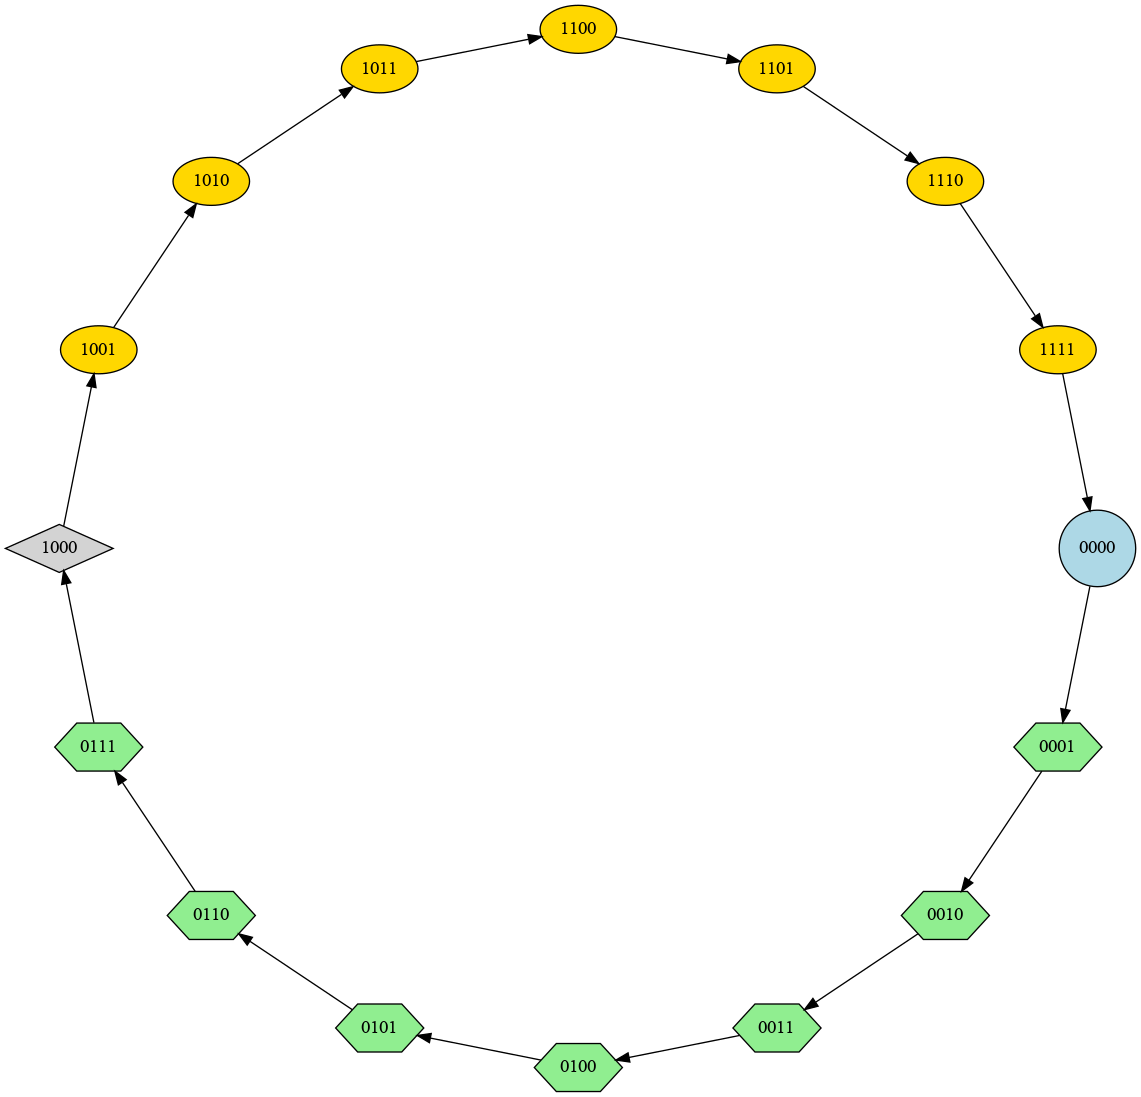
\includegraphics[scale=0.15]{../../Sources_images_logiques/images/cycle.png}
\caption{\label{fig:org3b73a8e}Relations entre les codes dans l'assignation en complément à deux}
\end{figure}
\end{frame}

\begin{frame}[label={sec:orgd4dfba8}]{Nombres signés et codage \ldots{} 2}
\begin{itemize}
\item En suivant cette logique, on pourra, comme indiqué sur la figure, assigner les codes en jaune à des valeurs positives et les codes en vert à des valeurs négatives.

\item Si on assigne autant de valeur positives que de valeurs négatives, un seul code binaire ne sera pas utilisable, le code 1000.

\item Tout mouvement selon le sens des flèches correspond à une addition; tout mouvement en sens inverse correspond à une soustraction.

\item Les nombres binaires seront ainsi symétriques par rapport à notre zéro.

\item Nous obtenons ainsi l'assignation du tableau \ref{tab:org936f239}.
\end{itemize}
\end{frame}

\begin{frame}[label={sec:org7fedabe}]{Nombres signés et codage \ldots{} 3}
\begin{columns}
\begin{column}{0.48\columnwidth}
\begin{block}{}
\begin{table}[htbp]
\caption{\label{tab:org936f239}Assignation de codes aux nombres de 4 bits}
\centering
\begin{tabular}{rr}
Code & Nombre\\
\hline
1001 & -7\\
1010 & -6\\
1011 & -5\\
1100 & -4\\
1101 & -3\\
1110 & -2\\
1111 & -1\\
\end{tabular}
\end{table}
\end{block}
\end{column}

\begin{column}{0.48\columnwidth}
\begin{block}{}
\begin{center}
\begin{tabular}{rr}
0000 & 0\\
0001 & 1\\
0010 & 2\\
0011 & 3\\
0100 & 4\\
0101 & 5\\
0110 & 6\\
0111 & 7\\
1000 & aucun\\
\end{tabular}
\end{center}
\end{block}
\end{column}
\end{columns}
\end{frame}

\begin{frame}[label={sec:org9d807c8}]{Nombres signés et codage \ldots{} 4}
\begin{itemize}
\item Voici quelques observations importantes sur cette représentation.

\begin{enumerate}
\item Tous les codes des nombres négatifs ont le premier bit à gauche (qui serait le bit le plus significatif) à la valeur 1, alors que les autres ont codes ont la valeur 0.

Ce bit peut ainsi servir d'indicateur de signe, avec la convention habituelle qu'on ne met pas de signe au zéro.

On parlera ainsi de \alert{bit de signe} pour dénoter ce bit, qui ne contribue pas à la grandeur (en valeur absolue) du nombre.
\end{enumerate}
\end{itemize}
\end{frame}

\begin{frame}[label={sec:orga1d1ad4}]{Nombres signés et codage \ldots{} 5}
\begin{enumerate}
\setcounter{enumi}{1}
\item L'inverse additif d'un nombre \(n\), c'est-à-dire \(-n\), est représenté par le \alert{complément à deux} du nombre.

Ceci signifie que pour trouver l'inverse additif d'un nombre, il suffit de calculer son complément à deux.

Le complément à deux du complément à deux nous re-donnera le nombre initial, conformément à la double négation \(--n = n\).
\end{enumerate}
\begin{itemize}
\item Il existe d'autres conventions pour la représentation de nombres signés, comme par exemple, la représentation signe+magnitude, mais la représentation en complément à deux est de loin la plus utilisée.
\end{itemize}
\end{frame}

\begin{frame}[label={sec:org23bcb4c}]{Opérations arithmétiques binaires: addition de nombres non signés}
\begin{itemize}
\item En transposant les opérations classiques pour effectuer à la main des additions ou des soustractions, il est possible d'effectuer des calculs avec des nombres binaires.

\item Additionner des nombres entier non signés ne pose pas de difficultés particulières.

\item On suppose deux nombre entiers binaires non signés \(A\) et \(B\) représentés en utilisant le même nombre de bits (si un nombre est plus petit, on ajoutera des 0 non significatifs à gauche pour compléter la représentation).
\end{itemize}
\end{frame}


\begin{frame}[label={sec:org219d010}]{Addition de nombres non signés \ldots{} 2}
\begin{itemize}
\item Lorsqu'on effectue l'opération bit par bit, en partant de la position la moins significative, on peut utiliser la table d'addition suivante:

\item À la position \(i\), on a trois entrées à prendre en considération: \(A_{i}\) et \(B_{i}\), les bits des nombres à additionner et \(R_{i-1}\), la retenue provenant de la position \(i-1\).

\item En sortie, on a la somme \(S_{i}\) et la retenue \(R_{i}\).
\end{itemize}
\end{frame}

\begin{frame}[label={sec:orgf3a6126}]{Addition de nombres non signés \ldots{} 3}
\begin{table}[htbp]
\caption{\label{tab:orgb7f07f3}Tableau de vérité pour l'additionneur binaire}
\centering
\begin{tabular}{rrrrr}
\(A_{i}\) & \(B_{i}\) & \(R_{i-1}\) & \(R_{i}\) & \(S_{i}\)\\
\hline
0 & 0 & 0 & 0 & 0\\
0 & 0 & 1 & 0 & 1\\
0 & 1 & 0 & 0 & 1\\
0 & 1 & 1 & 1 & 0\\
1 & 0 & 0 & 0 & 1\\
1 & 0 & 1 & 1 & 0\\
1 & 1 & 0 & 1 & 0\\
1 & 1 & 1 & 1 & 1\\
\end{tabular}
\end{table}
\end{frame}

\begin{frame}[label={sec:org164d2b3}]{Addition de nombres non signés: exemple 1}
Exemple:

A: 101110001
B: 001111001
S: 111101010
R: 001110001

S'il y a une retenue non nulle à la suite de l'addition à la position la plus significative, il y a un \alert{débordement}, car le résultat est trop grand pour être représenté avec le nombre de bits initial.
\end{frame}

\begin{frame}[label={sec:org3ae36c6}]{Addition de nombres signés \ldots{} 4}
\begin{itemize}
\item L'addition de nombre signés codés avec la représentation en complément à deux est nettement avantageuse.

\item Il suffit d’additionner les deux nombres comme s'il s'agissait de nombre non signés, en incluant les bits de signe dans le calcul.

\item La retenue qui émane de la position la plus significative ne doit pas être prise en compte.
\end{itemize}
\end{frame}

\begin{frame}[label={sec:orgcd7dbbe}]{Addition de nombres signés: exemple 2}
\begin{itemize}
\item Additionnons \(A=-2\) et \(B=4\), représentés respectivement (1110)2 et (0100)2.
\end{itemize}

A: 1110
B: 0100
S: 0010
R: 1100

qui nous donne bien le résultat escompté: S = (0010)2 = (2)10.
\end{frame}

\begin{frame}[label={sec:orgfead533}]{Addition de nombres signés: exemple 3}
\begin{itemize}
\item Additionnons \(A=3\) et \(B=-5\), représentés respectivement (0011)2 et (1011)2.
\end{itemize}

A: 0011
B: 1011
S: 1110
R: 0011

qui nous donne bien le résultat escompté: S = (1110)2 = (-2)10.
\end{frame}

\begin{frame}[label={sec:orgc91e2ed}]{Addition de nombres signés \ldots{} 5}
\begin{itemize}
\item On peut vérifier facilement qu'additionner un nombre avec son complément à deux donne toujours zéro, ce qui correspond à faire \(-n + n = 0\).

\item Comme avec l'addition de nombre entiers non signés, il faudra se préoccuper des débordements qui peuvent survenir parce que la capacité de représentation est limitée par la taille (en nombre de bits) des codes binaires utilisés.
\end{itemize}
\end{frame}

\begin{frame}[label={sec:orgd187f18}]{Soustraction de nombres signés}
\begin{itemize}
\item La soustraction s'effectue en faisant \(A - B = A + (-B)\), comme suit:

\begin{enumerate}
\item On détermine le complément à deux du nombre à soustraire (ici, \(B\)).
\item On additionne ce complément à deux au nombre duquel on soustrait  (ici, \(A\)).
\end{enumerate}

\item La retenue qui émane de la position la plus significative ne doit pas être prise en compte.

\item Le résultat s'interprétera comme un nombre signé en complément à deux.
\end{itemize}
\end{frame}

\begin{frame}[label={sec:orgdc33fed}]{Extension de signe}
\begin{itemize}
\item Dans la représentation des nombres signés en complément à deux, le bit de signe (bit le plus à gauche) est un indication directe du signe d'un nombre.

\item Si on change la taille des nombres, c'est-à-dire, le nombre de bits utilisés au total pour la représentation, il faut une opération spécifique pour préserver l'encodage en complément à deux.
\end{itemize}
\end{frame}

\begin{frame}[label={sec:orgf0ffbc1}]{Extension de signe \ldots{} 2}
\begin{itemize}
\item Considérons par exemple le nombre 5, représenté d'abord sur quatre bits et ensuite sur huit bits.
\end{itemize}

On a pour 5 $$ 0101 $$

ou encore $$ 00000101 $$

\begin{itemize}
\item Quand on compare ces deux représentations, on observe que: 

\begin{itemize}
\item elles se terminent de la même façon, avec les trois bits 101 qui représentent la grandeur du nombre;
\item le bit le plus à gauche est 0 dans les deux cas (même signe);
\item dans la représentation sur huit bits, il y a des bits 0 entre le bit  de signe et les trois derniers bits.
\end{itemize}
\end{itemize}
\end{frame}

\begin{frame}[label={sec:org9f97438}]{Extension de signe \ldots{} 3}
\begin{itemize}
\item Considérons maintenant un nombre négatif, le nombre -5, représenté d'abord sur quatre bits et ensuite sur huit bits.
\end{itemize}

Le complément à deux de 5 = (0101)2 est

$$ 1011 $$

alors que le complément à deux de 5 = (00000101)2 est $$ 11111011 $$

\begin{itemize}
\item Quand on compare ces deux représentations, on observe que: 

\begin{itemize}
\item elles se terminent de la même façon, avec les trois bits 011;
\item le bit le plus à gauche est 1 dans les deux cas (même signe);
\item dans la représentation sur huit bits, il y a des bits 1 entre le bit de signe et les trois derniers bits.
\end{itemize}
\end{itemize}
\end{frame}

\begin{frame}[label={sec:orgc9b304a}]{Extension de signe \ldots{} 4}
\begin{itemize}
\item Ces constatations nous amènent à conclure que lorsqu'on augmente la taille de représentation d'un nombre signé, il faut faire une \alert{extension de signe} pour intercaler les bonnes valeurs binaires entre le bit de signe et les bits qui représentent la grandeur du nombre.

\item Pour un nombre positif, on doit intercaler des bits 0, alors que pour un nombre négatif, on intercale des bits 1.

\item On peut donc énoncer la règle comme \emph{on doit intercaler des bits dont la valeur est la même que le bit de signe.}
\end{itemize}
\end{frame}

\begin{frame}[label={sec:org33c3a94}]{Extension de signe \ldots{} 5}
\begin{itemize}
\item Si, à l'inverse, on réduit la taille des nombres signés, on n'aura qu'à supprimer des bits, tous égaux au bit de signe, entre le bit de signe et ceux qui représentent la grandeur du nombre.

\item Si les bits à supprimer ne sont pas tous égaux au bit de signe, c'est une indication que la réduction de taille n'est pas possible: la nouvelle taille est insuffisante pour représenter les nombres correctement.
\end{itemize}
\end{frame}

\begin{frame}[label={sec:org92baaf5}]{Codes binaires}
\begin{itemize}
\item Il n'y a pas que des nombres que l'on voudra représenter en binaire.

\item Il est maintenant le temps de définir ce qu'on appelle un \alert{code binaire}, car cette notion est au centre de tous les encodages que nous aurons à utiliser.

\item Un code binaire sur \(n\) bits est typiquement une association entre, d'une part, les éléments d'un ensemble que l'on cherche à représenter et d’autre part, les différents groupes ou patrons possibles avec \(n\) bits.
\end{itemize}
\end{frame}

\begin{frame}[label={sec:org89edc83}]{Codes binaires \ldots{} 2}
\begin{itemize}
\item On appelle parfois ces patrons des mots-code (ou par abus de langage, des codes).

\item Comme il y a \(2^n\) patrons de bits différents, il est possible d'associer jusqu'à ce nombre d'éléments.

\item Une règle, souvent implicite mais essentielle, est qu'\alert{on ne devrait associer qu'un seul élément à un patron de bits donné.} Sinon, l'interprétation du code (le décodage) devient ambiguë.

\item Selon l'application, il n'est pas toujours nécessaire d'associer tous les patrons de bits à des éléments.
\end{itemize}
\end{frame}

\begin{frame}[label={sec:orgdeb7e8b}]{Codes binaires \ldots{} 3}
\begin{itemize}
\item Par exemple, si on veut représenter les chiffres décimaux, il est nécessaires de disposer d'au moins 10 patrons de bits, ce qui est possible avec \(n=4\).

\item Puisque \(2^4 = 16\), il y aura \(16 - 10 = 6\) patrons de bits inutilisés.

\item La règle spécifique d'association peut être établie arbitrairement, mais elle est souvent conçue en vue de respecter certaines propriétés liées aux éléments à représenter ou à la configuration du code lui-même.

\item C'est ce qu'on a fait, par exemple, pour définir la convention d'encodage des entiers par complément à deux.
\end{itemize}
\end{frame}

\begin{frame}[label={sec:org714ae00}]{Code Gray}
\begin{itemize}
\item Lorsqu'on utilise un code binaire pour représenter des valeurs associées à des phénomènes physiques, il peut être opportun d’utiliser un encodage dans lequel le nombre de changements de bits est minimal lorsqu'on passe d'un patron de bits au suivant dans la séquence des codes.

\item Par exemple, si on cherche à encoder des positions d'un interrupteur rotatif (comme pour encoder des angles), il est préférable que lorsqu'on passe d'un position à la suivante en tournant le commutateur, un seul bit ne change dans la sortie.

\item Ainsi, une erreur sur un bit n'introduit pas un gros changement dans l'interprétation de la valeur encodée.
\end{itemize}
\end{frame}

\begin{frame}[label={sec:orgb4f6c94}]{Code Gray \ldots{} 2}
\begin{itemize}
\item Un code Gray permet d'atteindre cet objectif.

\item Avec le code Gray du tableau \ref{tab:org59ec4cd}, on peut voir par exemple que la transition entre les codes pour 7 et 8 n’entraîne qu'un changement sur un bit, de 0110 à 1100.

\item Avec un encodage classique basé sur les entiers binaires, on aurait observé pour ce cas une transition entre 0111 et 1000, qui comporte quatre changements de valeurs de bits.
\end{itemize}
\end{frame}

\begin{frame}[label={sec:org265531e}]{Code Gray \ldots{} 3}
\begin{columns}
\begin{column}{0.48\columnwidth}
\begin{block}{}
\begin{table}[htbp]
\caption{\label{tab:org59ec4cd}Code Gray à quatre bits}
\centering
\begin{tabular}{rr}
Code Gray & Valeur\\
\hline
0000 & 0\\
0001 & 1\\
0011 & 2\\
0010 & 3\\
0110 & 4\\
0111 & 5\\
0101 & 6\\
0100 & 7\\
\end{tabular}
\end{table}
\end{block}
\end{column}


\begin{column}{0.48\columnwidth}
\begin{block}{}
\begin{center}
\begin{tabular}{rr}
Code Gray & Valeur\\
\hline
1100 & 8\\
1101 & 9\\
1111 & 10\\
1110 & 11\\
1010 & 12\\
1011 & 13\\
1001 & 14\\
1000 & 15\\
\end{tabular}
\end{center}
\end{block}
\end{column}
\end{columns}
\end{frame}


\begin{frame}[label={sec:org900d938}]{Codes alphanumériques et autres}
\begin{itemize}
\item Vous rencontrerez sans doute plusieurs autres encodages courants, comme par exemple pour encoder des caractères (code ASCII, codes UTF) ou pour encoder uniquement des chiffre décimaux (code BCD).

\item Une fois qu'on a bien compris la règle d'encodage, il n'y a généralement pas de difficultés à les utiliser.

\item Certains codes sont construits de manière à permettre d’identifier et même, dans certains cas, de corriger des erreurs dans le stockage ou la transmission des données encodées.

\item Ces codes sont construits en fonction de règles d'encodage, qui, lorsqu'elles ne sont pas respectées, permettent de constater la présence d'erreurs.
\end{itemize}
\end{frame}
\end{document}